\section{Theorie}
\label{sec:Theorie}

% TODO: ersten Satz überarbeiten
In diesem Versuch wird die Funktionsweise eines Reinst-Germanium-Detektors diskutiert
und verschiedene Proben anhand aufgenommener Spektren charakterisiert.
Dazu werden im Folgenden die verschiedenen Mechanismen zur Energiedeposition von
$\gamma$-Strahlung in Materie erläutert, der Aufbau eines Halbleiter-Detektors
dargestellt und ein typisches Spektrum einer $\gamma$-Quelle diskutiert.

Der Intensitätsverlust eines $\gamma$-Strahls in Materie ist abhängig von
der Schichtdicke des Materials, der Elektronendichte $n$ und dem
Wirkungsquerschnitt $\sigma$.
Letzter ist durch eine den Elektronen zugeordnete Fläche motiviert.
Diese Fläche lässt sich dann auf eine Wahrscheinlichkeit $W$ umrechnen,
mit welcher die Wechselwirkung eintritt. Für eine infinitesimale Schichtdicke
$\symup{d}x$ mit Gesamtfläche $F$ ergibt sich
\begin{equation*}
	\symup{d}W = \frac{n\:F\:\symup{d}x\:\sigma}{F} = n\:\sigma\:\symup{d}x
\end{equation*}
und nach Integration
\begin{equation}
	N\left(D\right) = N_\text{0} \cdot \exp^{-n\:\sigma\:D}
	\label{eqn:Intensitaet-Exp}
\end{equation}
mit der Schichtdicke $D$ und Anfangsintensität $N_\text{0}$.
Im Anschluss sind die Prinzipien und Wirkungsquerschnitte von drei
Wechselwirkungen näher betrachtet.

\subsection{Photo-Effekt}
\label{sec:Photo-Effekt}

Beim Photo-Effekt wechselwirkt ein Photon mit einem Hüllenelektron. Dabei
wird das Photon anhilliert und das Elektron verlässt die Atomhülle.
Hierzu muss die Energie des Photons also mindestens die Bindungsenergie des
Elektrons betragen.
Der nun unbesetzte Zustand in der Atomhülle wird durch ein Elektron aus
einem höheren Orbital besetzt, das dabei ein Photon mit charakteristischer
Energie emittiert. Die Lücke in dem höheren Orbital wird dann wiederum durch
ein Elektron aus einem noch höheren Orbital aufgefüllt und so weiter.

Der Wirkungsquerschnitt des Photo-Effekts ist abhängig von der Energie der
$\gamma$-Quanten und der Kernladungszahl $Z$.
Bei natürlichen Strahlern ergibt sich eine Abhängigkeit von
\begin{equation*}
	\sigma_\text{Ph} \sim Z^\alpha E^\delta
\end{equation*}
mit $4 < \alpha < 5$ und $\delta \approx \num{-3.5}$.
Für niedrige $\gamma$-Energien sind zudem Unstetigkeiten im Wirkungsquerschnitt
erkennbar, wenn die Energie genau der Ionisationsenergie einer Schale entspricht.

\subsection{Compton-Effekt}
\label{sec:Compton-Effekt}

Im Korpuskelmodell des Lichts kann der Compton-Effekt als unelastische
Streuung an einem Elektron aufgefasst werden.
Unter der Annahme eines ruhenden Elektrons lässt sich mit Hilfe von Impuls-
und Energieerhaltung die Energie des gestreuten $\gamma$-Quants zu
\begin{equation}
	E_{\gamma'} = E_\gamma
	\frac{1}{1 + \varepsilon \left(1 - \cos \psi_\gamma\right)}
	\label{eqn:Compton-Energy}
\end{equation}
mit der Abkürzung
\begin{equation*}
	\varepsilon \equiv \frac{E_\gamma}{m_\text{0}\:c^2}
\end{equation*}
berechnen.
Hierbei bezeichnet $m_0$ die Ruheenergie des Elektrons und
$c$ die Lichtgeschwindigkeit im Vakuum.
Der maximale Streuwinkel beträgt \SI{180}{\degree} bei einem maximalen
Energieübertrag an das Elektron von
\begin{equation*}
	E_\text{l,max} = E_\gamma \frac{2 \varepsilon}{1 + 2 \varepsilon} < E_\gamma.
\end{equation*}
Im Unterschied zum Photo-Effekt wird nur ein Teil der $\gamma$-Energie übertragen,
sodass nicht die gesamte Energie des Photons im Detektor deponiert werden muss und
das Photon den Detektor nach dem Compton-Effekt wieder verlassen kann.
Somit stellt der Compton-Effekt einen Störfaktor dar.

Von Interesse ist der differentielle Wirkungsquerschnitt nach der Energie der
Elektronen, da nur diese an den Detektor abgegeben wird. Hierzu
wird der Wirkungsquerschnitt für $\varepsilon \rightarrow 0$ betrachtet,
welcher durch
\begin{equation*}
	\sigma_\text{Compton} = \frac{3}{4} \sigma_\text{Th}
	= \frac{3}{4} \cdot \frac{8}{3} \pi
	\left(\frac{e_0}{4\:\pi\:\varepsilon_0\:c^2\:m_0}\right)^2
\end{equation*}
mit dem Thomsonschen Wirkungsquerschnitt $\sigma_\text{Th}$ gegeben ist.
Hierbei wurde angenommen, dass sich die Elektronen bei Anregung durch die
$\gamma$-Quanten wie Hertzsche Dipole verhalten.
Wird dieser Ausdruck nach der Energie abgeleitet, ergibt sich
\begin{equation}
	\frac{\symup{d}\sigma}{\symup{d}E} =
	\frac{3}{8} \sigma_\text{Th} \frac{1}{m_0\:c^2\:\varepsilon^2}
	\left\{2 + \left(\frac{E}{h \nu - E}\right)^2
	\left(\frac{1}{\varepsilon^2} + \frac{h \nu - E}{h \nu} - \frac{2}{\varepsilon}
	\left(\frac{h \nu - E}{h \nu}\right)\right)\right\}
	\label{eqn:Compton-Wirkungsquerschnitt}
\end{equation}
mit dem Planck'schen Wirkungsquantum $h$ und der Frequenz des $\gamma$-Quants $\nu$.
Der Verlauf dieses Wirkungsquerschnitts ist in Abbildung \ref{fig:Compton-Wirkungsquerschnitt}
dargestellt. Die sogenannte Compton-Kante kennzeichnet den maximalen Energieübertrag
$E_\text{l,max}$.

\begin{figure}
	\centering
	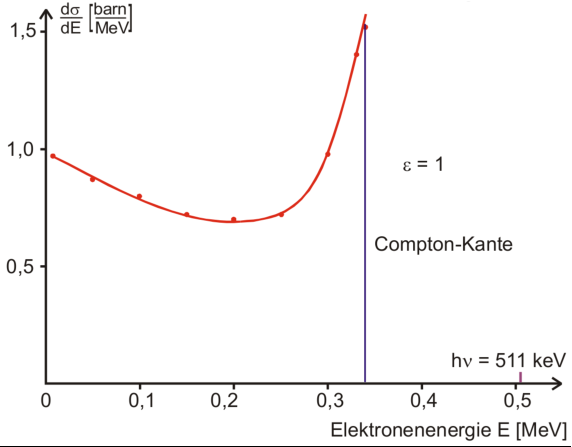
\includegraphics[height=7.0cm]{images/Compton-Wirkungsquerschnitt.pdf}
	\caption{Der differentielle Wirkungsquerschnitt nach \eqref{eqn:Compton-Wirkungsquerschnitt}
	in Abhängigkeit von der Elektronenenergie \cite[7]{anleitung}.}
	\label{fig:Compton-Wirkungsquerschnitt}
\end{figure}
% \FloatBarrier

\subsection{Paarerzeugung}
\label{sec:Paarerzeugung}



\subsection{Funktionsweise eines Halbleiter-Detektors}
\label{sec:HLDetektor}

\subsection{Spektrum, Aktivität und Energie einer Gamma-Quelle}
\label{sec:TypischeQuelle}

